\documentclass[compress]{beamer}
\mode<presentation>
\setbeamercovered{transparent}
\usetheme{Warsaw}
%\useoutertheme{smoothtree}
\usepackage{multirow}
\usepackage[english]{babel}
\usepackage[latin1]{inputenc}
\usepackage{times}
\usepackage[T1]{fontenc}
\usepackage{xmpmulti}
\usepackage{multicol}
\usepackage{colortbl}

%\setbeamersize{text margin left=.25 in,text margin right=.25 in}
\setbeamersize{text margin left=.15 in,text margin right=.15 in}
\usepackage[authoryear]{natbib}


\usepackage{epstopdf}
\usepackage{xcolor}
\usepackage{latexcolors}
%\usepackage[dvipsnames]{xcolor}
\definecolor{antiquebrass}{rgb}{0.8, 0.58, 0.46}
\definecolor{babyblueeyes}{rgb}{0.63, 0.79, 0.95}
\definecolor{babyblue}{rgb}{0.54, 0.81, 0.94}
\definecolor{bistre}{rgb}{0.24, 0.17, 0.12}
\definecolor{brightlavender}{rgb}{0.75, 0.58, 0.89}
\definecolor{bulgarianrose}{rgb}{0.28, 0.02, 0.03}
\definecolor{slateblue}{rgb}{0.56, 0.74, 0.56}
\definecolor{cordovan}{rgb}{0.54, 0.25, 0.27}
\definecolor{darkbyzantium}{rgb}{0.36, 0.22, 0.33}

\setbeamercolor{structure}{fg=airforceblue!80, bg= black!60}







\usepackage{tikz}
\usetikzlibrary{shadows,calc}
\usetikzlibrary{shadows.blur}
\usetikzlibrary{shapes.symbols}
\usepackage{hyperref}
\usepackage{booktabs}
\usepackage{colortbl}
\usepackage{multirow}
%%%%%%%%% shaddow image %%%%%
% some parameters for customization
\def\shadowshift{3pt,-3pt}
\def\shadowradius{6pt}
\colorlet{innercolor}{black!60}
\colorlet{outercolor}{gray!05}
% this draws a shadow under a rectangle node
\newcommand\drawshadow[1]{
\begin{pgfonlayer}{shadow}
    \shade[outercolor,inner color=innercolor,outer color=outercolor] ($(#1.south west)+(\shadowshift)+(\shadowradius/2,\shadowradius/2)$) circle (\shadowradius);
    \shade[outercolor,inner color=innercolor,outer color=outercolor] ($(#1.north west)+(\shadowshift)+(\shadowradius/2,-\shadowradius/2)$) circle (\shadowradius);
    \shade[outercolor,inner color=innercolor,outer color=outercolor] ($(#1.south east)+(\shadowshift)+(-\shadowradius/2,\shadowradius/2)$) circle (\shadowradius);
    \shade[outercolor,inner color=innercolor,outer color=outercolor] ($(#1.north east)+(\shadowshift)+(-\shadowradius/2,-\shadowradius/2)$) circle (\shadowradius);
    \shade[top color=innercolor,bottom color=outercolor] ($(#1.south west)+(\shadowshift)+(\shadowradius/2,-\shadowradius/2)$) rectangle ($(#1.south east)+(\shadowshift)+(-\shadowradius/2,\shadowradius/2)$);
    \shade[left color=innercolor,right color=outercolor] ($(#1.south east)+(\shadowshift)+(-\shadowradius/2,\shadowradius/2)$) rectangle ($(#1.north east)+(\shadowshift)+(\shadowradius/2,-\shadowradius/2)$);
    \shade[bottom color=innercolor,top color=outercolor] ($(#1.north west)+(\shadowshift)+(\shadowradius/2,-\shadowradius/2)$) rectangle ($(#1.north east)+(\shadowshift)+(-\shadowradius/2,\shadowradius/2)$);
    \shade[outercolor,right color=innercolor,left color=outercolor] ($(#1.south west)+(\shadowshift)+(-\shadowradius/2,\shadowradius/2)$) rectangle ($(#1.north west)+(\shadowshift)+(\shadowradius/2,-\shadowradius/2)$);
    \shade[outercolor,right color=innercolor,left color=innercolor] ($(#1.north west)+(-\shadowradius/12,\shadowradius/12)$) rectangle ($(#1.south east)+(\shadowradius/12,-\shadowradius/12)$);%Frame
    \filldraw ($(#1.south west)+(\shadowshift)+(\shadowradius/2,\shadowradius/2)$) rectangle ($(#1.north east)+(\shadowshift)-(\shadowradius/2,\shadowradius/2)$);
\end{pgfonlayer}
}
% create a shadow layer, so that we don't need to worry about overdrawing other things
\pgfdeclarelayer{shadow} 
\pgfsetlayers{shadow,main}
% Define image shadow command
\newcommand\shadowimage[2][]{%
\begin{tikzpicture}
\node[anchor=south west,inner sep=0] (image) at (0,0) {\includegraphics[#1]{#2}};
\drawshadow{image}
\end{tikzpicture}}
\usepackage{calligra}

\DeclareMathOperator*{\argmax}{Arg\,max}
\DeclareMathOperator*{\argmin}{Arg\,min}
\newcommand{\norm}[1]{\left\Vert #1 \right\Vert }
\newcommand{\bbetaHat}{ \widehat{\bbeta}}
\newcommand{\bbetaLSE}{ \widehat{\bbeta}_{_{\text{LSE}}}}
\newcommand{\bbetaMLE}{ \widehat{\bbeta}_{_{\text{MLE}}}}
\newcommand{\sqBullet}[1]{  {\tiny \tiny \tiny \qBoxCol{#1!60}{ }} }
%***************
%\newtheorem{thm}{Theorem}
%\documentclass[noinfoline]{imsart}
%\usepackage{amsmath,amstext,amssymb}
%%\usepackage[top=1.5in, bottom=1.5in, left=1.2in, right=1.2in]{geometry}
%% settings
%%\pubyear{2005}
%%\volume{0}
%%\issue{0}
%%\firstpage{1}
%%\lastpage{8}
%\arxiv{arXiv:0000.0000}

%\startlocaldefs
%\numberwithin{equation}{section}
%\theoremstyle{plain}
%\newtheorem{thm}{Theorem}
%\endlocaldefs
\usepackage{lipsum} 
\usepackage{amsmath}
\usepackage{amssymb}
\usepackage{amsbsy} 
\usepackage{amsthm}
\usepackage{mathrsfs}
\usepackage{eufrak}
\usepackage{mathrsfs}
\usepackage{color}
\usepackage{verbatim}
\usepackage{graphicx}
\usepackage{bm}
\usepackage{enumerate}
\usepackage{epstopdf} 
\usepackage{natbib}
\usepackage{undertilde}
%\RequirePackage[colorlinks,citecolor=blue,urlcolor=blue]{hyperref}
%\usepackage{subfig}
\usepackage[final]{pdfpages}

\usepackage{algorithm}  %@subhajit
\usepackage{algpseudocode} %@subhajit
\usepackage{algorithmicx}     %@subhajit
\usepackage{undertilde}


\newcommand{\sphere}{{\mathbb{S}}}
\newcommand{\R}{\mathbb{R}}
\newcommand{\LatentV}{V}
\newcommand{\NC}{m}
\newcommand{\Priorf}{f_{prior}}
\newcommand{\FWOne}[2]{{{}_{1}\Psi _{1}\left[{\begin{matrix}(\frac{#1}{2},\frac{1}{2})\\(1,0)\end{matrix}};#2\right]} 
}


\newcommand{\HyPriorMu}{\thetabf}
\newcommand{\HyPriorAlpha}{\alpha}
\newcommand{\HyPriorBeta}{\beta}
\newcommand{\HyPriorK}{\zeta}
\newcommand{\Indicator}[2]{\mathbb{I}_{_{#1}}({#2 })}
\newcommand{\xb}{\bm{x}}
\newcommand{\bx}{\MakeVec{\bm{x}}}
\newcommand{\bX}{\bm{X}}
\newcommand{\by}{\MakeVec{\bm{y}}}
\newcommand{\bZ}{\bm{Z}}
\newcommand{\bF}{\bm{F}}
\newcommand{\btheta}{\MakeVec{{\bm{\theta}}}}
\newcommand{\Bpi}{\MakeVec{\boldsymbol{\pi}}}
\newcommand{\thetabf}{\MakeVec{\boldsymbol{\theta}}}
\newcommand{\Thetabf}{\boldsymbol{\Theta}}
\newcommand{\taubf}{\MakeVec{\boldsymbol{\tau}}}
\newcommand{\Tr}{Tr}


\newcommand{\bM}{\bm{M}}
\newcommand{\bD}{\MakeVec{\bm{D}}}
\newcommand{\bV}{\MakeVec{\bm{V}}}
\newcommand{\loglikmix}{\mathcal{L}_{\bM,\bD,\bV}}
\newcommand{\hypdc}{{}_0F_1\left(\frac{n}{2},\frac{D_c^2}{4}\right)}


\usepackage{xstring}
\usepackage[normalem]{ulem}
\definecolor{ultramarine}{RGB}{38,29,163}
\newcommand\PalDel[1]{{\color{red} {\sout{#1}}}}
\newcommand\Pal[1]{{\color{ultramarine}{#1}}}
\newcommand\PalRp[2]{\PalDel{#1} \Pal{#2}}
\newcommand\PalCmnt[1]{{\color{ultramarine} {[[[***PAL:  #1 ***]]]}}}

\newcommand{\qedwhite}{\hfill \ensuremath{\Box}}
\newcommand{\SpaceD}{\mathcal{S}_p}
\newcommand{\SpaceM}{\widetilde{\mathcal{V}}_{n,p}}
\newcommand{\SpaceV}{\mathcal{V}_{p,p}}
\newcommand{\SpaceF}{\mathbb{R}^{n,p}}
\newcommand{\StiefelS}{\mathcal{V}_{n,p}}
\newcommand{\SpacePi}{\mathbb{S}_{\pi}}
\newcommand{\ML}{{\cal{ML}}}
\newcommand{\ProdSpace}{\boldsymbol{\Theta}}
\newcommand{\ThetaAndPi}{\Xi}
\newcommand{\ClassML}{\mathcal{C}_{\ML}}


\newcommand{\balpha}{\MakeVec{\bm{\alpha}}}
\newcommand{\bbeta}{\MakeVec{\bm{\beta}}}
\newcommand{\bEta}{\bm{\eta}}
\newcommand{\bd}{{\utilde{\bm{d}}}}
\newcommand{\BoEta}{{\utilde{\boldsymbol{\eta}}}}
%\newtheorem{theorem}{Theorem}[section]
%\newtheorem{theorem}{Theorem}
%\newtheorem{lemma}{Lemma}
%\newtheorem{result}{Result}
\newtheorem{defn}{Definition}
\newcommand{\pdv}[2][]{\frac{\partial#1}{\partial#2}}
\newcommand{\pdvtwo}[2][]{\frac{\partial^2#1}{{\partial#2}^2}}


%\newcommand{\mubf}{\boldsymbol{\mu}}
\newcommand{\mubf}{\MakeVec{\mu}}
\newcommand{\sumI}{ \sum_{i=1}^{n}}
\newcommand{\Ybar}{{\overline{Y}}}

\newcommand{\Expectation}[1]{\mathbb{E}{[#1]}}
\newcommand{\priorXzero}{\Psi}
\newcommand{\iMat}{\mathbf{I}_{p}}

% 
% \newtheorem{thm}{Theorem}[section]
% \newtheorem{cor}[thm]{Corollary}
% \newtheorem{lem}[thm]{Lemma}
%\newtheorem{proposition}{Proposition}

%\newtheorem{theorem}{Theorem}[chapter]%To link the theorem to each chapter uncomment the chapter option
%\newtheorem{lemma}{Lemma}%[theorem]% To link each lemma to a theorem uncomment the theorem option
%\newtheorem{corollary}{Corollary}%[theorem]% To link each corollary to a theorem uncomment the theorem option
% to link a corollary to a chapter change the theorem option to chapter
%\newtheorem{definition}{Definition}%[chapter] %the same is true for both definitions and assumptions
\newtheorem{assumption}{Assumption}%[chapter] %
%\newtheorem{proposition}{Proposition}[chapter]
%\newtheorem{fact}{Fact} %%% added by @subho
\newcommand{\StrongNBD}[2]{S_{#1}{#2}}
\newcommand{\bpi} {\boldsymbol{\pi}}
\newcommand{\bphi} {\boldsymbol{\phi}}
\newcommand{\bb}[1]{\boldsymbol{#1}}
% Definitions of handy macros can go here

\newcommand{\normtwo}[1]{{\left\lVert#1\right\rVert}_2}

\newcommand{\dataset}{{\cal D}}
\newcommand{\fracpartial}[2]{\frac{\partial #1}{\partial  #2}}
\newcommand{\Lesbegue}[1]{\mu_{\btheta_{#1},\bpi_{#1}}}
\newcommand{\fthetapi}[1]{f_{\btheta_{#1},\bpi_{#1}}}
% Heading arguments are {volume}{year}{pages}{submitted}{published}{author-full-names}
\newcommand{\doublehat}[1]{%
    \settoheight{\dhatheight}{\ensuremath{\widehat{#1}}}%
    \addtolength{\dhatheight}{-0.35ex}%
    \widehat{\vphantom{\rule{2pt}{\dhatheight}}%
    \smash{\hspace{-0.5mm}\widehat{#1}}}}

\newcommand{\hyp}{{}_0F_1\left(\frac{n}{2},\frac{D^2}{4}\right)}
\newcommand{\hypinline}{{}_0F_1\left({n}/{2},{D^2}/{4}\right)}

\newcommand{\partialhyp}[1]{\frac{\partial}{\partial\,{d_{#1}}}\,\left[\hyp\right]}

\newcommand{\fracProbZ}[1]{\frac{\langle Z_{ic} \rangle \, #1}{\sum_{i=1}^{N} \langle Z_{ic}\rangle  } }
\newcommand{\EmVar}[1]{\widetilde{#1}^{(c)}}

\newcommand{\IMDY}{{\it{CCPD}}}
\newcommand{\JMDY}{{\it{JCPD}}}

\newcommand{\DYlang}{\frac{\exp(\nu\,\bEta^T\bd)}{{\left[{}_0F_1\left(\frac{n}{2},\frac{D^2}{4}\right)\right]}^{\nu}}}

\newcommand{\logDYlang}{\nu\,\bEta^T\bd - \nu\,\log\left({}_0F_1\left(\frac{n}{2},\frac{D^2}{4}\right)\right)}

\newcommand{\lhyp}{\log\left({}_0F_1\left(\frac{n}{2},\frac{D^2}{4}\right)\right)}

%\jmlrheading{1}{2000}{1-48}{4/00}{10/00}{SS \& JH \& AB}

% Short headings should be running head and authors last names

%\ShortHeadings{BDP and cIBP}{SS \& JH \& AB}
%\firstpageno{1}

\newcommand{\diam}[1]{{{#1}^{\ast}}}

%%% coloring option %%%
\definecolor{auburn}{rgb}{0.53, 0.1, 0.5}
\newcommand{\sss}{\color{auburn}}  %%% for Subhajit
\newcommand{\sse}{\color{black}}
\newcommand{\attn}{\color{red}}
\newcommand{\rms}{\color{magenta}}  %%% for Riten
\newcommand{\rme}{\color{black}}
\newcommand{\MLDensity}{f_{\ML}}
\setlength{\parindent}{0cm}
\newcommand{\posterior}

\newcommand{\variableX}{\bd}
\newcommand{\funch}{\mathfrak{h}}
\newcommand{\IndVzero}[1]{\mathbb{I}({X\in \mathcal{V}^{#1}_0})}
\newcommand{\Rnp}{\mathbb{R}^{n \times p}}
\newcommand{\Rpp}{\mathbb{R}^{p \times p}}
\newcommand{\vecnorm}[1]{\lVert #1\rVert}

\newcommand{\etapsiD}{\eta_{\priorXzero}}
\newcommand{\BoEtapsiD}{\BoEta_{\priorXzero}}

\newcommand{\DMp}{\mathcal{D}^{p \times p}}
\newcommand{\Rplus}{\mathbb{R}_{+}}
\newcommand{\prodMeasure}{\Upsilon}

\newcommand{\m}{{\bf m_{\BoEta}}} 
\newcommand{\SetWithMode}{\mathcal{S}}
\newcommand{\SetWithModePrime}{\mathcal{S}}
\newcommand{\TargetComp}{\mathcal{S}^{\star}}

\newcommand{\ConstCondDen}{K_{\nu, \BoEta}} 

\newcommand{\hyparam}[2]{
    \IfEqCase{#1}{
        {M}{\xi^{#2}_c}
        {V}{\gamma^{#2}_c}%
        
    }
  }
\newcommand{\threepartdef}[6]
{
	\left\{
		\begin{array}{lll}
			#1 & \mbox{if } #2 \\
			#3 & \mbox{if } #4 \\
			#5 & \mbox{if } #6
		\end{array}
	\right.
}

\def\bv{\color{blue}}
\def\ev{\color{black}}
\newcommand{\bch}{\bv }
\newcommand{\ech}{\ev\normalsize}
%\newcommand{\MakeVec}[1]{{\utilde{\bf #1}}}
\newcommand \Measure[2][]{%
  \ifstrempty{#1}{
  \IfEqCase{#2}{
        {M}{\mu}%
        {D}{\mu_1}%
        {V}{\mu_2}
        {X}{\mu}
   }  
  }{
  \IfEqCase{#1}{
  {1}{
   \IfEqCase{#2}{
        {M}{d\mu(M)}%
        {D}{d\mu_1(\bd)}%
        {V}{d\mu_2(V)}
        {X}{d\mu(X)}
        {Y}{d\mu(Y)}
        {MDV} {d\mu(M)\; d\mu_1(\bd) \;d\mu_2(V) }
        }
   } 
   {2}{
   \IfEqCase{#2}{
         {M}{d\mu(M^{\ast})}%
        {D}{d\mu_1(\bd^{\ast})}%
        {V}{d\mu_2(V^{\ast})}
        {X}{d\mu(X^{\ast})}
        }
   }
   {3}{
   \IfEqCase{#2}{
         {M}{\mu(dM^{\star})}%
        {D}{\mu_2(d\bd^{\star})}%
        {V}{\mu_1(dV^{\star})}
        {X}{\mu(X^{\star})}
        }
   }   
   
   } 
  }%
}
  \newcommand{\VONF}{\text{VonMisesFisher}}
\newcommand{\MPGalpha}{\alpha}
\newcommand{\MPGnu}{\nu}
\newcommand{\MPG}{MPG }
\newcommand{\ybin}{y^{(\text{bin})}}


%\newcommand{\abs}[1]{\left \vert  #1  \right\vert  }
\usepackage{caption}
\usepackage{subcaption}

%%%%%%%%%%%%%%%%%%%%%%%%%%%
\newcommand{\IEHC}{\text{IEHC}}







\newcommand \Th[1]{%
  \IfEqCase{#1}{
        {1}{ 1^{\text{st}}}%
        {2}{2^{\text{nd}}}%
        {3}{3^{\text{rd}}}%
  }[{#1}^{\text{th}}]
}
  
  
   \newcommand{\augV}{\text{aux}}
  
  
  
  
  \newcommand{\CDE}{\text{PL}}
\newcommand{\CDEsigma}{\sigma}
\newcommand{\CDEepsilon}{\SVepsilon}
\newcommand{\CDEmu}{\mu}
 % \newcommand{\SVepsilon}{\varepsilon}
  \newcommand{\SVepsilon}{\delta}
 \newcommand{\abs}[1]{\left\lvert{#1}\right \rvert }
 
 
\newcommand{\CPDX }{\text{CPDX}}
\newcommand{\CPDXPar}{\vartheta}
\newcommand{\K}{\mathcal{K}}



\newcommand{\lossFunctionOne}[1]{ \left\{ \abs{ ( \abs{#1}-\SVepsilon)}  + ( \abs{#1}-\SVepsilon)\right\} }

\newcommand{\lossFunctionAlt}[1]{ \abs{  #1-\SVepsilon}  + \abs{ #1+\SVepsilon}-2\SVepsilon }

\newcommand{\lossFunctionAltOne}[1]{   \lossFunctionAlt{ \frac{\left(#1\right)}{\sigma}}}

\newcommand{\lossFunction}[1]{ \left\{ \abs{ \left( \frac{\abs{#1}}{\sigma}-\SVepsilon\right)}  + \left( \frac{\abs{#1}}{\sigma}-\SVepsilon\right)\right\} }
\newcommand{  \Likelihood}{\mathcal{L}}
%\newcommand{\Onebf}{\bf 1}
\newcommand{\Onebf}{{\bf \utilde{1}_{n}}}





\newcommand{\InvGamma}{\text{InvGamma}}
\newcommand{\PriorSigmaAlpha}{a}
\newcommand{\PriorSigmaBeta}{b}
\newcommand{\PriorBetaMean}{\mubf_{_{\bbeta}}}
\newcommand{\PriorBetaVar}{\Sigma_{_{\bbeta}}  }
\newcommand{\mvnormPdf}[4]{\frac{1}{ \left({2\pi}\right)^{\frac{#4}{2}} \sqrt{\vert{#3}\vert}}{\exp\left[ - \frac{1}{2}(#1- #2)^T {#3}^{-1} (#1- #2)\right]}      }
\newcommand{\InvGammaPdf}[3]{ \frac{(#1)^{-#2+1}}{\Gamma\left( #2\right) } \exp\left[ -\frac{{#3}}{{#1}} \right] }

 \newcommand{\byTilde}{\tilde{\by}}
 
 \newcommand{\TrfSigma}{\varsigma}
 \newcommand{ \Normal}{\text{Normal}}
 \newcommand{\GlobalPar}{\tau}
\newcommand{\LocalPar}{\psi}
\newcommand{\Not}[1]{{\overline{#1}}}
\newcommand{\st}{:}

\newcommand{\define}[2]{ \begin{definition}[#1]  #2  \end{definition}  }

\newcommand{\Exmpl}[2]{\qBrd[0.75in]{#1}{Example #2:}}
\newcommand{\Qn}{\HLTW{Question:} }


\newcommand{\pmf}{p}
\newcommand{\cdf}{F}
%\NewDocumentCommand{\support}{O{ }}{{\mathcal{S}}_{_{#1}}}
\NewDocumentCommand{\support}{O{ }}{{\mathbb{S}}_{_{#1}}}
%\newcommand{\SampleS}{\mathcal{S}}
\newcommand{\SampleS}{\mathscr{S}}
\usepackage{xcolor}
\usepackage{xparse}
\definecolor{lightGray}{gray}{0.95}
\definecolor{lightGrayOne}{gray}{0.9}
\definecolor{lightBlueOne}{RGB}{204, 255, 255}
\definecolor{lightBlueTwo}{RGB}{204, 238, 255}
\definecolor{lightBlueThree}{RGB}{204, 204, 255}
\definecolor{AltBlue}{RGB}{119,14,161}
\definecolor{Orchid}{RGB}{186,85,211}

\definecolor{BGBlue}{RGB}{220,221,252}
\definecolor{BGBlueOne}{RGB}{204,229,255}

\definecolor{DarkGreenOne}{RGB}{34,139,34}

\definecolor{BGGreen}{RGB}{240,243,245}
\definecolor{lightGreenOne}{RGB}{179, 255, 179}
\definecolor{lightGreenTwo}{RGB}{198, 255, 179}
\definecolor{lightGreenThree}{RGB}{243, 255, 230}
\definecolor{AltGreen}{RGB}{193, 240, 240}

\definecolor{BOGreen}{RGB}{180,0,0}
\definecolor{BGGreenOne}{RGB}{220,250,220}

\definecolor{lightBrownOne}{RGB}{255, 221, 204}
\definecolor{lightBrownTwo}{RGB}{255, 229, 204}
\definecolor{lightBrownThree}{RGB}{242, 217, 230}


\definecolor{HLTGreen}{RGB}{230,244,215}
\definecolor{ExcBrown}{RGB}{153,0,0}
\definecolor{ExcBGBrown}{RGB}{255,204,204}
\definecolor{BGYellowOne}{RGB}{255,235,208}
\definecolor{BGPink}{RGB}{255,215,240}

\newcommand{\MakeVec}[1]{{\utilde{\bf #1}}}

\NewDocumentCommand{\MCOption}{O{1.75in} m}{
\TextInBoxTwo[BGPink]{ #1 } {\TextInBoxTwo[white]{.1 in }{ \quad}\HLT{#2}}
}

 \NewDocumentCommand{\ThreeChoices}{O{Do not Know}O{Not confident}O{Confident}}{
\MCOption{#1} \MCOption{#2} \MCOption{#3}
}
 
\NewDocumentCommand{\OneBlock}{ O{HLTGreen} m m }{\colorbox{#1}{\begin{minipage}{#2} $ #3$ \end{minipage}}}

\NewDocumentCommand{\HLT}{ O{HLTGreen} m }{\colorbox{#1}{#2}}
%\NewDocumentCommand{\HLTEQ}{ O{HLTGreen} m }{\colorbox{#1}{$#2$}}
\NewDocumentCommand{\HLTEQ}{ O{white} m }{\colorbox{#1}{$#2$}}

%\newcommand{\HLT}[1]{\colorbox{HLTGreen}{#1}}
\newcommand{\DEHLT}[1]{\colorbox{lightGrayOne}{\color{white} #1}}

\newcommand{\TextInBoxOne}[2]{  {\fcolorbox{white}{lightGrayOne}{\begin{minipage}{#1}  #2 \end{minipage}}}}


\NewDocumentCommand{\TextInBoxTwo}{ O{lightGrayOne} m m } {{\fcolorbox{white}{#1}{\begin{minipage}{#2} { #3} \end{minipage}}}}


\newcommand{\TextInBox}[2]{  {\fcolorbox{BGGreen}{BGGreen}{\begin{minipage}{#1}  #2 \end{minipage}}}}
\newcommand{\TextInBoxCol}[2]{
\fcolorbox{BGBlue}{BGBlue}{%
\begin{minipage}{#1}
 {\color{AltBlue} #2}
\end{minipage}}%
}

\NewDocumentCommand{\TxtBnd}{ O{lightBrownOne} m m } {{\fcolorbox{white}{#1}{\begin{minipage}{#2} { #3} \end{minipage}}}}


\newcommand{\BandInTopBox}[2]{
\fcolorbox{AltBlue}{AltBlue}{%
\begin{minipage}{#1}{ {\color{white}  #2 \hspace{.1in}} }
\end{minipage}}%
}


\newcommand{\TextInBoxThm}[2]{
\fcolorbox{AltBlue}{lightGray}{%
\begin{minipage}{#1}
 {\color{black} #2}
\end{minipage}}%
}

\newcommand{\TextInBoxThmOne}[2]{
\fcolorbox{BGBlue}{BGBlueOne}{%
\begin{minipage}{#1}
 {\color{AltBlue} #2}
\end{minipage}}%
}

\newcommand{\TextInBoxLem}[2]{
\fcolorbox{BGBlue}{lightGray}{%
\begin{minipage}{#1}
 {\color{black} #2}
\end{minipage}}%
}



\newcommand{\TextInBoxLemOne}[2]{
\vspace{.02 in}
\noindent
\fcolorbox{BGBlue}{BGBlue}{%
\begin{minipage}{#1}
 {\color{AltBlue} #2}
\end{minipage}}%
}



\newcommand{\DefBox}[1]{
%\vspace{.1 in}
\noindent
\TextInBoxLem{4.5 in }{
\BandInTopBox{4.4 in }{}
\TextInBoxLemOne{4.4 in }{
#1
}}}





\newcommand{\DefBoxOne}[2]{
%\vspace{.1 in}
\noindent
\TextInBoxLem{4.5 in }{
\BandInTopBox{4.4 in }{#1}
\TextInBoxLemOne{4.4 in }{
#2
}}}


\newcommand{\ThmBox}[2]{
\noindent
\TextInBoxThm{4.4 in }{
\TextInBoxThmOne{4.4 in }{
#1}
#2}
}

\newcommand{\LemBox}[2]{
\noindent
\TextInBoxLem{4.5 in }{
\TextInBoxLemOne{4.4 in }{
#1}
#2}
}

\newcommand{\PropBox}[2]{
\vspace{.1 in}
\noindent
\TextInBoxLem{4.5 in }{
\TextInBoxLemOne{4.4 in }{
#1}
#2}
}




\newcommand{\TextInBoxExc}[2]{
\noindent
\fcolorbox{white}{BGGreenOne}{%
\begin{minipage}{#1}
 {\color{black} #2}
\end{minipage}}%
}


\newcommand{\TextInBoxExample}[2]{
\noindent
\fcolorbox{white}{BGPink}{%
\begin{minipage}{#1}
 {\color{black} #2}
\end{minipage}}%
}


\newcommand{\ExerciseBox}[1]{
\noindent
%\TextInBoxLem{6 in }{
\TextInBoxExc{6 in }{
#1}
%#2}
}


\newcommand{\ExampleBox}[1]{
\noindent
%\TextInBoxLem{6 in }{
\TextInBoxExample{6 in }{
#1}
%#2}
}

\NewDocumentCommand{\CommentBox}{ O{BGBlue}  m }{
\TextInBoxLem{5.5in }{
{\bf Comment:}\\
\TextInBoxLemOne{5.4 in }{
#2}}
}



\newcommand{\HLTY}[1]{\HLTEQ[yellow]{#1}}
\newcommand{\HLTW}[1]{\HLTEQ[white]{#1}}



\newcommand{\qBox}[1]{
  \begin{tikzpicture}
\node[draw=none,shade,
      top color=lightGrayOne,
      bottom color=lightGray,
      rounded corners=2pt,
      blur shadow={shadow blur steps=5}
    ] at (0,0) {    \noindent 
\fcolorbox{white}{BGBlue}{%
\begin{minipage}{4.55 in}
 {\color{black} {
 #1}}
\end{minipage}  }%
 };
 
    \end{tikzpicture}
}
 
 


 

\newcommand{\qBoxCol}[2]{
  \begin{tikzpicture}
\node[draw=none,shade,
      top color=lightGrayOne,
      bottom color=lightGray,
      rounded corners=2pt,
      blur shadow={shadow blur steps=5}
    ] at (0,0) {    \noindent
\fcolorbox{white}{#1}{%
%\begin{minipage}{4.55 in}
\begin{minipage}{4.55 in}
 {
 \color{black} {
 #2}}
\end{minipage}  }%
 };
 
    \end{tikzpicture}
}
  
  
  
  
  
  

\NewDocumentCommand{\qBrd}{O{4.55 in} m m}{
  \begin{tikzpicture}
\node[draw=none,shade,
      top color=#2,
      bottom color=#2,
      rounded corners=2pt,
      blur shadow={shadow blur steps=5}
    ] at (0,0) {    \begin{minipage}{#1}
 {
 \color{black} {
 #3}}
\end{minipage} 

 };
 
    \end{tikzpicture}
}
    
  
  
  
  
\NewDocumentCommand{\qbx}{O{4.55 in} m m}{
  \begin{tikzpicture}
\node[draw=none,shade,
      top color=lightGrayOne,
      bottom color=lightGray,
      rounded corners=2pt,
      blur shadow={shadow blur steps=5}
    ] at (0,0) {    \noindent
\fcolorbox{white}{#2}{%
%\begin{minipage}{4.55 in}
\begin{minipage}{#1}
 {
 \color{black} {
 #3}}
\end{minipage}  }%
 };
 
    \end{tikzpicture}
}
  
 
 
 \newcommand{\CurlyBox}[1]{
\begin{center}
  \begin{tikzpicture}
    \node[tape,draw=none,shade,
      top color=blue!40,
      bottom color=blue!5,
      rounded corners=1pt,
      blur shadow={shadow blur steps=5,shadow blur extra rounding=1.3pt}
    ] at (2,0){\sffamily\bfseries\large #1};
  \end{tikzpicture}
\end{center} 
 }


\newcommand{\CmntBnd}{\BandInTopBox{4.5in}{Comment:}}
\NewDocumentCommand{\TopBand}{O{Comment:} m}{ \BandInTopBox{4.5in}{#2}}

\newcommand{\DBX}[1]{
 	\HLTEQ[AltBlue]{
 				\HLTEQ[BGBlue]{  #1  }
 	}
 }



\NewDocumentCommand{\TransitionFrame}{O{slateblue}m}{
\begin{frame}{ }
\qBoxCol{#1!40}{\vspace{.8in}  \begin{center}\qBrd[2in]{#1!70}{ \begin{center} \vspace{.1in}
  #2 \\
 \vspace{.1in}
\end{center}}\end{center}
\vspace{.7in}
}

\end{frame}

}


\newcommand \rbind[1]{%
    \saveexpandmode\expandarg
    \StrSubstitute{\noexpand#1}{,}{&}[\fooo]%
    %\StrSubstitute{\fooo}{,}{&}[\fooo]%
    \StrSubstitute{\fooo}{;}{\noexpand\\}[\fooo]%
    \StrSubstitute{\fooo}{:}{\noexpand\\}[\fooo]%
    \restoreexpandmode
   \left[ \begin{matrix}\fooo\end{matrix}\right]
    }
    
    
    
   \newcommand \ColVec[1]{%
    \saveexpandmode\expandarg
    \StrSubstitute{\noexpand#1}{,}{\noexpand\\}[\fooo]%
    %\StrSubstitute{\fooo}{,}{&}[\fooo]%
    \StrSubstitute{\fooo}{;}{\noexpand\\}[\fooo]%
    \StrSubstitute{\fooo}{:}{\noexpand\\}[\fooo]%
    \restoreexpandmode
   \left[ \begin{matrix}\fooo\end{matrix}\right]
    }
     \newcommand \RowVec[1]{%
    \saveexpandmode\expandarg
    \StrSubstitute{\noexpand#1}{,}{&}[\fooo]%
    %\StrSubstitute{\fooo}{,}{&}[\fooo]%
    \StrSubstitute{\fooo}{;}{&}[\fooo]%
    \StrSubstitute{\fooo}{:}{&}[\fooo]%
    \restoreexpandmode
   \left[ \begin{matrix}\fooo\end{matrix}\right]
    }



  \newcommand \Row[1]{%
    \saveexpandmode\expandarg
    \StrSubstitute{\noexpand#1}{,}{&}[\fooo]%
    %\StrSubstitute{\fooo}{,}{&}[\fooo]%
    \StrSubstitute{\fooo}{;}{&}[\fooo]%
    \StrSubstitute{\fooo}{:}{&}[\fooo]%
    \restoreexpandmode
    \begin{matrix}\fooo\end{matrix}
    }
        
    
    
    
    \newcommand \Col[1]{%
    \saveexpandmode\expandarg
    \StrSubstitute{\noexpand#1}{,}{\noexpand\\}[\fooo]%
    %\StrSubstitute{\fooo}{,}{&}[\fooo]%
    \StrSubstitute{\fooo}{;}{\noexpand\\}[\fooo]%
    \StrSubstitute{\fooo}{:}{\noexpand\\}[\fooo]%
    \restoreexpandmode
    \begin{matrix}\fooo\end{matrix}
    }

%%%%%%%%%%%%%%%%%%%%% Experimental %%%%%%%%%%%%%%%%%


\ExplSyntaxOn
\DeclareExpandableDocumentCommand{\replicate}{O{}mm}
 {
  \int_compare:nT { #2 > 0 }
   {
    {#3}\prg_replicate:nn {#2 - 1} { #1#3 }
   }
 }
\ExplSyntaxOff


\ExplSyntaxOn
\DeclareExpandableDocumentCommand{\repdiag}{O{}mm}
 {
  \int_compare:nT { #2 > 0 }
   {
    {\prg_replicate:nn {#2}{#3#1}}{#3}
   }
 }
\ExplSyntaxOff


\newcommand \StrRowDiag[1]{%
    \saveexpandmode\expandarg
    \StrSubstitute{\noexpand#1}{,}{&}[\fooo]%
    %\StrSubstitute{\fooo}{,}{&}[\fooo]%
    \StrSubstitute{\fooo}{;}{&}[\fooo]%
    \StrSubstitute{\fooo}{:}{&}[\fooo]%
    \StrCount{\fooo}{&}[\countfooo]
    \restoreexpandmode
    \repdiag[0]{\countfooo+1}{{,}}
   %\left[ \begin{matrix}\fooo\end{matrix}\right]
    }


\newcommand \DiagStrOne[2]{%
    \saveexpandmode\expandarg
    \StrSubstitute{\noexpand#1}{,}{\noexpand#2}[\fooo]%
    \restoreexpandmode
   %\left[ \begin{matrix}\fooo\end{matrix}\right]
   \fooo
    }
    
    \newcommand \DiagStr[1]{%
    \DiagStrOne{#1}{{\StrRowDiag{#1}}}
    }


%$\rbind{\replicate[,]{10}{\Col{\replicate[;]{7}{0}}}}$

%$\Col{1,2,3}$
%$\ColVec{\replicate[;]{5}{B}}$
%$ \StrRowDiag{1,2} $

%$\DiagStr{1,2,3}$

%\repdiag[-]{3}{A}
\ExplSyntaxOn
\NewDocumentCommand{\Split}{ m m o }
 {
  \tarass_split:nn { #1 } { #2 }
  \IfNoValueTF { #3 } { \tl_use:N } { \tl_set_eq:NN #3 } \l_tarass_string_tl
 }

\tl_new:N \l_tarass_string_tl

\cs_new_protected:Npn \tarass_split:nn #1 #2
 {
  \tl_set:Nn \l_tarass_string_tl { #2 }
  % we need to start from the end, so we reverse the string
  \tl_reverse:N \l_tarass_string_tl
  % add a comma after any group of #1 tokens
  \regex_replace_all:nnN { (.{#1}) } { \1\, } \l_tarass_string_tl
  % if the length of the string is a multiple of #1 a trailing comma is added
  % so we remove it
  \regex_replace_once:nnN { \,\Z } { } \l_tarass_string_tl
  % reverse back
  \tl_reverse:N \l_tarass_string_tl
 }
\ExplSyntaxOff

%%%%%%%%%%%%%%%%%%%%%%%%%%%%%%%%

\newcommand{\ShowRowMatrix}[3]{ \left[ {\begin{array}{ccc}
  \line(1,0){22} &{#1} &  \line(1,0){22} \\
     & \vdots& \\
  \line(1,0){22}  &{#2}& \line(1,0){22} \\
   &  \vdots & \\
    \line(1,0){22} &{#3}& \line(1,0){22}  \\
    \end{array}
   } \right]}
 


\newcommand{\ShowColMatrix}[3]{ \left[ {\begin{array}{ccccc}
  \line(0,1){25} & &\line(0,1){25} &  &  \line(0,1){25} \\
  {#1}  & \ldots & {#2} &\ldots   &{#3} \\
 \line(0,1){25} &  & \line(0,1){25}  &  &  \line(0,1){25} \\
    \end{array}
   } \right]}
   
   
   
   
\newcommand{\ShowRowVector}[1]{ \left[ {\begin{array}{ccc}
  \line(1,0){25} &{#1} &  \line(1,0){25} 
    \end{array}
   } \right]}   
   
   
\newcommand{\ShowColVector}[1]{ \left[ {\begin{array}{c}
  \line(0,1){25} \\    {#1} \\   \line(0,1){25}     \end{array}  } \right]}
  
\newcommand{\ColVector}[3]{ \left[ {\begin{array}{c}
  {#1}\\ \vdots \\    {#2}\\ \vdots\\{#3}  \end{array}  } \right]}
  
  
  
  
  
\newcommand{\EqSetThree}[3]{ \left\{ {\begin{array}{c}
  {#1}\\ \vdots \\    {#2}\\ \vdots\\{#3}  \end{array}  } \right.}  
  



\newcommand{\MatrixTypeA}[3]{ \left[ {\begin{array}{ccc}
 {#1}_{1,1} & \cdots & {#1}_{1,{#3}}   \\
  {#1}_{2,1} & \cdots & {#1}_{2,{#3}}   \\
    \vdots  & \ddots& \vdots  \\
     {#1}_{{#2},1} & \cdots & {#1}_{{#2},{#3}}   \\
    \end{array}
   } \right]}
 
\newcommand{\MatrixTypeAKronecker}[4]{ \left[ {\begin{array}{ccc}
 {#1}_{11}{#4} & \cdots & {#1}_{1{#3}}{#4}   \\
  {#1}_{21} {#4} & \cdots & {#1}_{2{#3}} {#4}   \\
    \vdots  & \ddots& \vdots  \\
     {#1}_{{#2}1} {#4} & \cdots & {#1}_{{#2}{#3}} {#4}   \\
    \end{array}
   } \right]}
 



\newcommand{\ShowIMat}{ {\begin{array}{cccc}
 1&  &  &    \\
  & 1 &  &  \\
    &  & \ddots &    \\
     & & & 1   \\
    \end{array}
   } }
 
\newcommand{\ShowVecOne}{
\begin{array}{c}
 1\\ 1 \\    1  
\end{array}
}

 
\newcommand{\ShowUnitVecOne}{
\begin{array}{c}
 1\\ 0 \\   0  
\end{array}
}


\newcommand{\ShowUnitVecTwo}{
\begin{array}{c}
 0\\ 1 \\   0  
\end{array}
}


\newcommand{\ShowUnitVecThree}{
\begin{array}{c}
 0\\ 0\\   1  
\end{array}
}

\newcommand{\ShowZeroThree}{
\begin{array}{c}
 0\\ 0\\   0 
\end{array}
}


\newcommand{\TwoBlockMatrix}[2]{\left[  {\begin{array}{c;{2pt/2pt}c}
   {#1} &  {#2}
   \end{array} }\right]}
   
   \newcommand{\TwoBlockMatrixH}[2]{\left[  {\begin{array}{c}
   {#1} \\
   \hdashline[2pt/2pt]
    {#2}
   \end{array} }\right]}
   
   \newcommand{\TwoBlockH}[2]{ {\begin{array}{c}
   {#1} \\
   \hdashline[2pt/2pt]
    {#2}
   \end{array} }}
   
   
\newcommand{\TwoBlock}[2]{ {\begin{array}{c;{2pt/2pt}c}
   {#1} &  {#2}
   \end{array} }}
   

      
   
   
   
 \newcommand{\ThreeBlockColVec}[3]{
   \left[ {\begin{array}{c}
  #1\\
  \hdashline[2pt/2pt]\\
   \vdots\\
  \hdashline[2pt/2pt]\\
  #2\\
  \hdashline[2pt/2pt]\\
   \vdots\\
  \hdashline[2pt/2pt]\\
   #3\\
    \end{array}
   } \right]
   }



\NewDocumentCommand{\ColDyn}{>{\SplitList{;}}m}
   {
     \left[\begin{array}{c}
       \ProcessList{#1}{ \inserColtitem }
     \end{array}\right]
   }
   \newcommand \inserColtitem[1]{ #1 \\}


\makeatletter
\newcommand{\ColDynAlt}[2][r]{%
  \gdef\@VORNE{1}
  \left[\hskip-\arraycolsep%
    \begin{array}{#1}\vekSp@lten{#2}\end{array}%
  \hskip-\arraycolsep\right]}

\def\vekSp@lten#1{\xvekSp@lten#1;vekL@stLine;}
\def\vekL@stLine{vekL@stLine}
\def\xvekSp@lten#1;{\def\temp{#1}%
  \ifx\temp\vekL@stLine
  \else
    \ifnum\@VORNE=1\gdef\@VORNE{0}
    \else\@arraycr\fi%
    #1%
    \expandafter\xvekSp@lten
  \fi}
\makeatother


\NewDocumentCommand{\eVec}{m O{}}{\MakeVec{e}_{#1, (#2)}}

\NewDocumentCommand{\Ones}{O{3}}{\Col{\replicate[,]{#1}{1}}}
\NewDocumentCommand{\Zeros}{O{3}}{\Col{\replicate[,]{#1}{0}}}











\title{  STAT 320: Principles of Probability\\ {\color{black} \HLTW{ \text{Unit 6} \HLTY{\text{Part:C}}}\\ The Normal Distribution}}

\author[UAEU]
{United Arab Emirates University}
\institute[UAEU] % (optional, but mostly needed)
{
  \inst{Department of Statistics}%
  %Indian Institute of Management,  Udaipur\\
  \vspace{0.1in}

  
}

\date{}


\newcommand{\Xnew}{ \HLTEQ[orange]{X_{_{\text{i}}}} }
\newcommand{\Ynew}{ \HLTEQ[orange]{Y_{_{\text{i}}}} }

%\date{\today}

\AtBeginSection[]
{
  \begin{frame}{Inhalt}
 % \begin{multicols}{1}
	\frametitle{Outline}
    \tableofcontents[currentsection]
  %  \end{multicols}
  \end{frame}
}

\begin{document}
\maketitle

%\begin{frame}{Outline}
%%\begin{multicols}{}
%  \tableofcontents
%%\end{multicols}
%\end{frame}

%\section{Introduction to DSBA 2023}
%
%
%\begin{frame}
%\qBoxCol{blue!30}{
%\begin{center} Course  Website \end{center}
%\qbx[4.2in]{teal!40}{\sqBullet{teal} \color{blue} $ \href{https://sites.google.com/iimu.ac.in/dsba2023e/home}{https://sites.google.com/iimu.ac.in/dsba2023e/home}$
%}\\
%\qbx[3.0in]{green!40}{ \sqBullet{green} Regular Announcements.
%}\\
%\qbx[3.0in]{olive!40}{\sqBullet{olive}  Slides and other materials.
%}
%}
%
%\pause
%\qBoxCol{blue!30}{
%\sqBullet{blue}
%You can contact the instructor at {\it subhadip.pal@iimu.ac.in} and schedule for office hours.  
%}
%\pause
%\qBoxCol{olive!30}{
%\sqBullet{olive}
%Mr. Praveen Kumar has been assigned as Teaching Assistant (TA) for this course.  His email I'd is:  {\it praveen.kumar@iimu.ac. }
%}
%
%
%\end{frame}
%


%
%\begin{frame}{Course Outline}
%\hspace{-.1in}\qBoxCol{blue!35}{
%% Please add the following required packages to your document preamble:
%% \usepackage{booktabs}
%\begin{table}[]
%\begin{tabular}{@{}lll@{}}
%\toprule
%         & Topics                                                & Dataset or Case                                    \\ \midrule \midrule
%\rowcolor{blue!20}     \multicolumn{1}{|l|}{1-2}   & \multicolumn{1}{l|}{Overview of Data Science}        & \multicolumn{1}{l|}{Household Data}                \\ \midrule
%\rowcolor{purple!20} 
%\multicolumn{1}{|l|}{3-5}   & \multicolumn{1}{l|}{Data Visualization}              & \multicolumn{1}{l|}{Global Super Store }       \\ \midrule
%\rowcolor{blue!20} 
%\multicolumn{1}{|l|}{6}     & \multicolumn{1}{l|}{Introduction to R/ JMP}          & \multicolumn{1}{l|}{}                              \\ \midrule
%\rowcolor{purple!20} 
%\multicolumn{1}{|l|}{7}     & \multicolumn{1}{l|}{Regression Analysis}             & \multicolumn{1}{l|}{Display \& Liquor Sales} \\ \midrule
%\rowcolor{blue!20} 
%\multicolumn{1}{|l|}{8}     & \multicolumn{1}{l|}{Multiple Regression}             & \multicolumn{1}{l|}{}                              \\ \midrule
%\rowcolor{purple!20} 
%\multicolumn{1}{|l|}{9}     & \multicolumn{1}{l|}{Dealing with Nominal Covariates} & \multicolumn{1}{l|}{Gender Divide}                 \\ \midrule
%\rowcolor{blue!20} 
%\multicolumn{1}{|l|}{10}    & \multicolumn{1}{l|}{Regression Diagonistics}         & \multicolumn{1}{l|}{}                              \\ \midrule
%\rowcolor{purple!20} 
%\multicolumn{1}{|l|}{11-12} & \multicolumn{1}{l|}{Project Presentations}            &\multicolumn{1}{l|}{}          \\\midrule \bottomrule
%\end{tabular}
%\end{table}
%}
%\end{frame}


%\begin{frame}{Case Study }
%\qBoxCol{teal!40}{\vspace{1in}\begin{center}\sqBullet{teal} \Large Case: Liquor sales and display space \end{center}
%\vspace{1in}
%}\\
%\end{frame}




%\section{A Few Widely Used Continuous Probability Distributions}
%\TransitionFrame[airforceblue]{\Large A Few Widely Used Continuous Probability Distributions  }


\section{$\Phi(\cdot):  $ Standard Normal CDF}


\TransitionFrame[bittersweet]{\Large $\HLTW{\Phi\left(x \right)\text{ Function}, } ${\tiny $x\in \R$ }\\The Standard Normal CDF }

\begin{frame}\frametitle{The Standard Normal CDF ( PHI function)  $\Phi(x)$, $x\in \R$.}

\begin{center}
\qBrd[4.5in]{applegreen!40}{ $\HLTW{\HLTY{\Phi\left(\HLTEQ[amethyst!40]{x} \right)}:= \displaystyle \int\limits_{-\infty}^{\HLTEQ[amethyst!40]{x} }  \frac{1}{\sqrt{2\pi }}e^{-\frac{z^2}{2}} dz} $ for all $x\in \R$.}
\vspace{.35in}
 \end{center}
\vspace{2in}
\end{frame}



\begin{frame}\frametitle{The Standard Normal CDF ( PHI function)  $\Phi(x)$, $x\in \R$.}
%\begin{center}
%\qBrd[4.5in]{white!40}{ }
%\vspace{.4in}
\begin{itemize}
\qBrd[1in]{carolinablue!50}{ \item $\HLTY{\Phi(0)}=\frac{1}{2}$}

\qBrd[4.2in]{camel!50}{ \item  $\HLTW{\HLTY{\Phi(-x)}+\HLTY{\Phi(x)}=1} \implies \HLTW{ \HLTY{\Phi(-x)}= 1-\HLTY{ \Phi(x)} }$ for all $x\in \R$}

\qBrd[3.2in]{celadon!50}{ \item  $\HLTW{0 \leq \HLTY{\Phi(x)} \leq 1}$ }

\qBrd[3.2in]{candypink!50}{ \item $\HLTW{\displaystyle \lim\limits_{x\rightarrow -\infty} \HLTY{\Phi(x)}=0}$, and  $\HLTW{\displaystyle \lim\limits_{x\rightarrow \infty} \HLTY{\Phi(x)}=1}$}
 \end{itemize}
 %\end{center}
\vspace{2in}
\end{frame}



\section{Normal Distribution}

\TransitionFrame[airforceblue]{\Huge Normal Distribution }


\begin{frame}
The normal distribution is one of the most commonly used probability distribution for applications:
\begin{itemize}
\item  When we repeat an experiment numerous times and average our results, the random variable representing the average or total tends to have a normal distribution as the number of experiments becomes large.
\item   The previous fact, which is known as the central limit theorem, is fundamental to many of the statistical techniques we will discuss later.
\item  Many physical characteristics (Heights, weights, etc.) tend to follow a normal distribution.
\item  Errors in measurement or production processes can often be
approximated by a normal distribution.
\item Under certain conditions, many probability distributions can be
approximated by a normal distribution.
\end{itemize}
\end{frame}



\begin{frame}
The Normal Distribution denoted by $\text{Normal}(\mu, \sigma^2)$ is characterized by two parameters, namely the mean $\mu\in \R$ and the standard deviation $\sigma>0$.
\define{Normal Distribution}{ A continuous random variable X is said to be normally distributed with mean $\mu\in \R$ and variance $\sigma^2>0$,  if its probability density function is given as 
$$\HLTW{ \displaystyle    f(x)= \frac{1}{\sigma \sqrt{2\pi}} e^{-\frac{(x-\mu)^2}{2\sigma^2}}}  \text{ for } -\infty <x<\infty. $$
}
\qBrd{applegreen!40}{
If $X\sim $ Normal($\mu, \sigma^2$) then 
$\HLTW{E(X) =\mu \text{ and }, \text{Var}(X) = \sigma^2}$
}


\end{frame}





\begin{frame}
\qBrd[4.6in]{ceil!50}{
\begin{center}
\Large 
Let $X\sim \text{Normal}(\mu, \sigma^2)$ for $\mu\in \R, \sigma^2>0$
\end{center}
}\\
\vspace{.5in}

%\qBrd[4.6in]{babyblue!40}{
$\Row{\qBrd[.9in]{amethyst!50}{\text{Mean}\\
\HLTW{E(X)= \mu } \vspace{.2in}},  \qBrd[1.73in]{amethyst!50}{\text{Variance}\\\HLTW{\text{VAR}(X)= \sigma^2  }\vspace{.2in}}  , \qBrd[1.5in]{amethyst!50}{\text{MGF}\\\HLTW{\text{M}_{_X}(t)= e^{\mu t +\frac{t^2\sigma^2}{2}} } \vspace{.2in}} } $
%}

\vspace{.1in}
\qBrd[4.6in]{antiquefuchsia!50}{
\begin{center}
\qBrd[4.2in]{white!40}{
{
\tiny
\begin{tabular}{|c|c|c|c|c|c|}
\hline
 Distribution & Support  &  pdf    & Mean   &  Variance  & mgf   \\
& $\support[X]$  &   $f_{_X}(x)$   &  $E(X)$  &   $\text{Var}(X)$  &  $M_{_X}(t)$  \\
 \hline \hline
 & & & & & \\
 $\text{Normal}(\mu, \sigma^2 )$&$ (-\infty , \infty )$ & $  \frac{1}{\sigma\sqrt{2\pi}}e^{-\frac{(x-\mu)^2}{2\sigma^2}} $ & $\mu  $  & $\sigma^2 $&   $  e^{\mu t +\frac{t^2\sigma^2}{2}}$\\
 $\HLTW{\text{mean}= \mu, \text{Variance}}= \sigma^2$ & & $\text{ for  } x\in \R $ & & & \\
 \hline
  \hline
\end{tabular}
}}\end{center}}
\end{frame}


\begin{frame}{Intuitive Understanding of the Parameters of a Normal Random Varibles }

\end{frame}





\begin{frame}
\qBrd{amber!20}{\vspace{-.2in}
\begin{center}
\qBrd[2.2in]{amber!70}{\begin{center}\Large Standard Normal \\ $\HLTW{\text{Normal}(\mu=0, \sigma^2=1)}$\end{center}}
\end{center}
\vspace{-.1in}
 Normal($0, 1$),(i.e. Normal distribution with mean $\mu=0$ and variance $\sigma^2=1$,) is referred to as the  {\bf  Standard Normal} Distribution. 
}\\
\vspace{.1in}
\qBrd{babyblue!40}{
\qBrd[1.5in]{babyblue!70}{Z-Transformation } 
 If $X\sim \text{Normal}(\mu, \sigma^2)$ for some $\mu\in \R$ and $\sigma^2>0$ then , 
 $$\DBX{\HLTW{ \Large Z \sim \text{Normal}(0,1) }\text{where } \HLTY{\Large Z= \frac{X-\mu}{\sigma}}}$$
}


\end{frame}



\begin{frame}{The role of the parameters $\mu$ and $\sigma^2$}

\end{frame}


\begin{frame}\frametitle{Finding Probabilities Using Normal CDF}
The cdf of the normal distribution,  does not have a closed form analytical expression and the corresponding integral is nontrivial to evaluate. 

The same is true for the cdf of the standard normal distribution (commonly denoted by $\Phi(z)$). However, $\Phi(z)$ is usually tabulated for values of z from -3.49 to 3.49 in increments of 0.01 and can be usedto calculate any normal probability by standardizing it first.

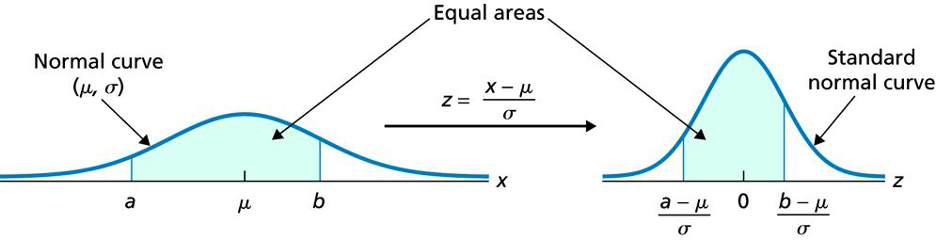
\includegraphics[scale=.6]{figs/NormalCDFStandardization.png}
\end{frame}





\begin{frame}\frametitle{Example}
%\tiny
\vspace{-.1in}
\qbx[4.6in]{olive!40}{
\Exmpl{olive}{} The times of first failure of a unit of a brand of ink jet printers are approximately normally distributed with a mean of 1,500 hours and a standard deviation of 200 hours. Use the statistical calculator.
\begin{enumerate}[a).]
\item What fraction of these printers will fail before 1,000 hours?
\item What is the probability that the first failure time of a selected printer will fail be between 1,300 and 1700 hours?
\end{enumerate}
}\\
%\pause
\vspace{2in}
\end{frame}





\begin{frame}\frametitle{Example}
$X\sim\text{Normal}(\mu= 1500, \sigma^2=200^2)$.\\
{\tiny 
\begin{minipage}{.45\textwidth} %
{\small 
 \qBrd[2.4in]{babyblueeyes!40}{
 \begin{eqnarray}
& &  P(X<1000)\nonumber\\
 & = &P\left(\HLTY{ \frac{X-\mu}{\sigma}} <\frac{1000-\mu}{\sigma}\right) \nonumber\\
  & = &P\left(\HLTY{Z} <\frac{1000-1500}{200}\right) \nonumber\\
    & = &P\left(\HLTY{Z} <-2.5\right) \nonumber\\
   & =& \Phi(-2.5) \nonumber\\
   & =&0.0062\nonumber
 \end{eqnarray}
 }}
\end{minipage} % 
\hspace{.1in}
\begin{minipage}{.45\textwidth} %
{\tiny 
 %\qBrd[2.1in]{babyblue!40}{\begin{center}
 %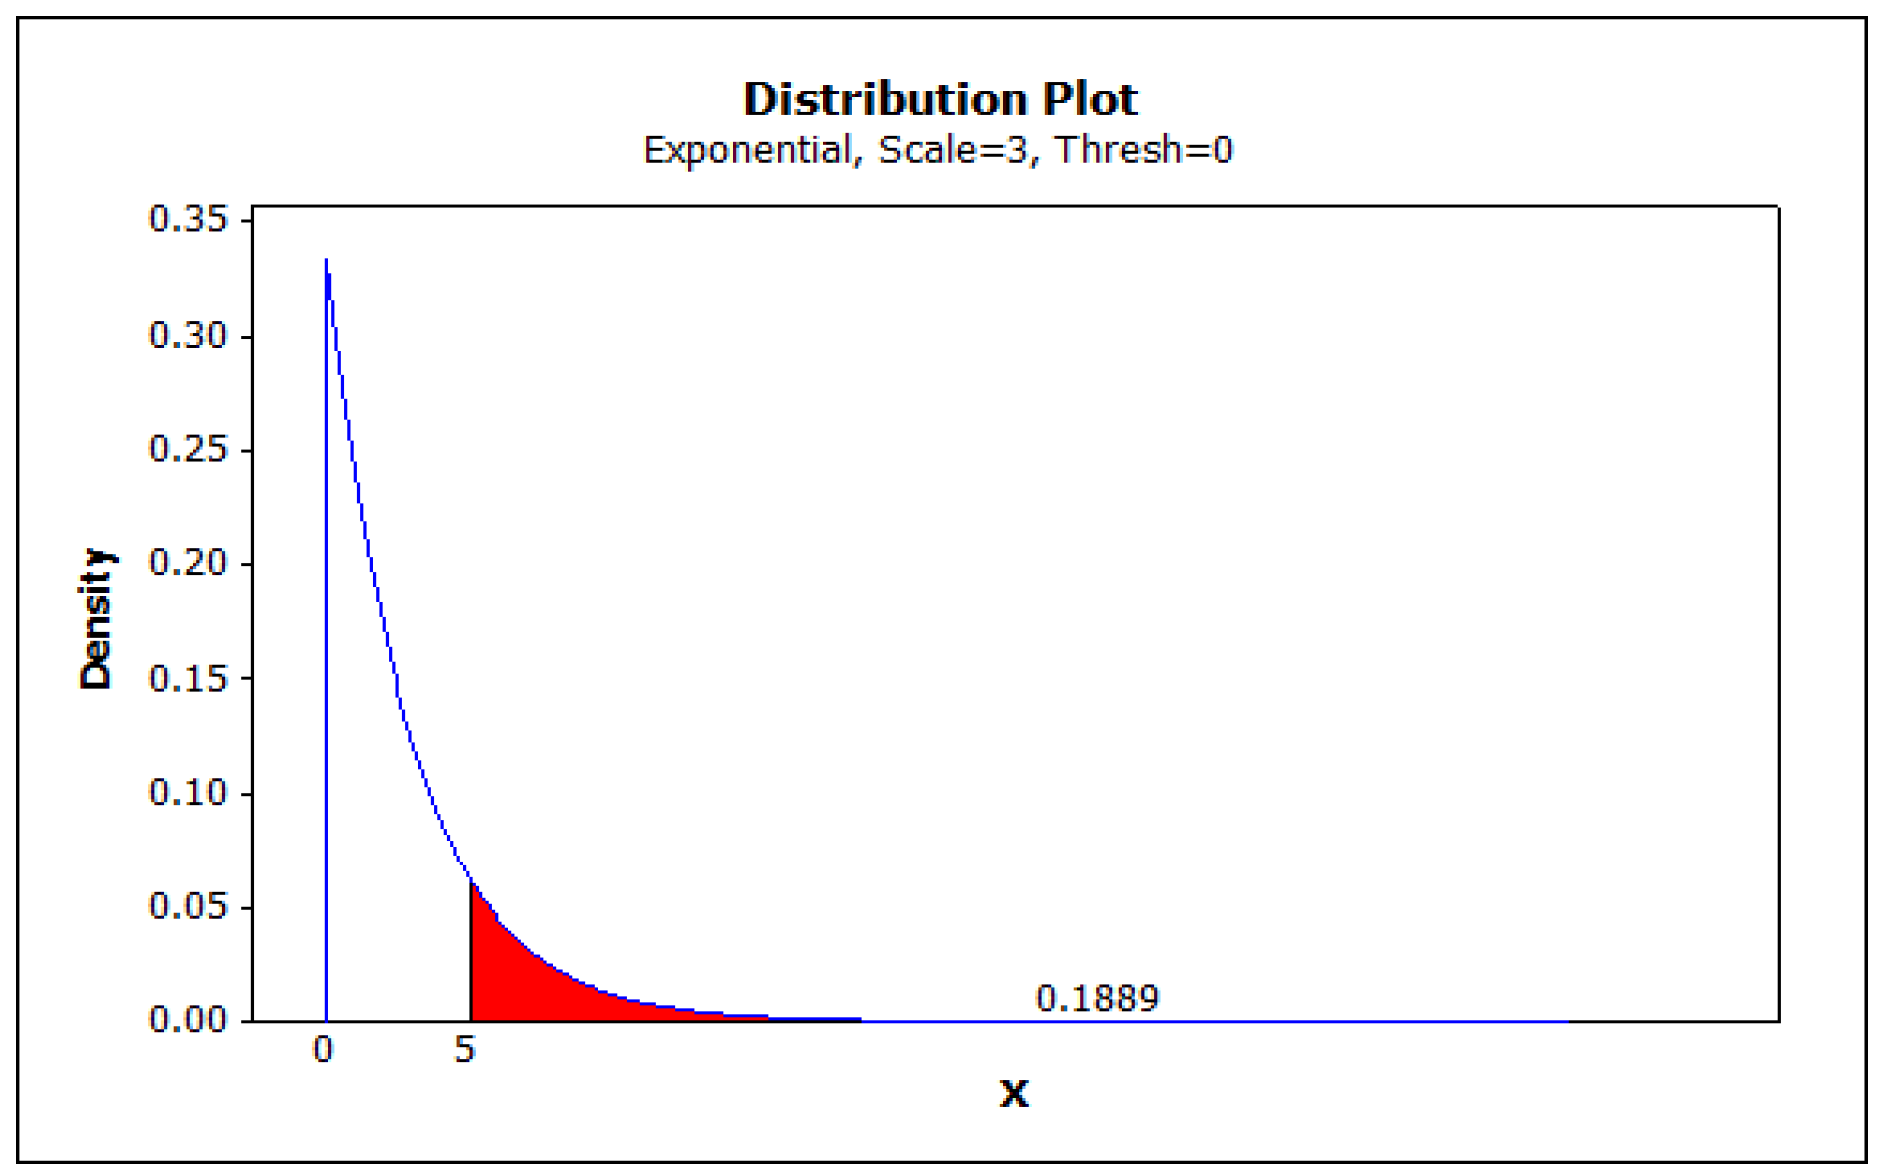
\includegraphics[scale=.15]{figs/pdf_Exponential_density2.png}
% \end{center}
 %}
 }
\end{minipage}
}
\end{frame}


\begin{frame}\frametitle{Example}
$X\sim\text{Normal}(\mu= 1500, \sigma^2=200^2)$.\\
{\tiny 
\begin{minipage}{.45\textwidth} %
{\small 
 \qBrd[3in]{babyblueeyes!40}{
 \begin{eqnarray}
& &  P(1300<X<1700)\nonumber\\
 & = &P\left(\frac{1300-\mu}{\sigma}<\HLTY{ \frac{X-\mu}{\sigma}} <\frac{1700-\mu}{\sigma}\right) \nonumber\\
  & = &P\left(\frac{1300-1500}{200}<\HLTY{Z} <\frac{1700-1500}{200}\right) \nonumber\\
    & = &P\left(-1<\HLTY{Z} <-1\right) \nonumber\\
   & =& \Phi(1)-\Phi(-1) \nonumber\\
   & =&  0.8413 -0.1587  \nonumber\\
   & =&  0.6826  \nonumber
 \end{eqnarray}
 }}
\end{minipage} % 
\hspace{.1in}
\begin{minipage}{.45\textwidth} %
{\tiny 
% \qBrd[2.1in]{babyblue!40}{\begin{center}
% %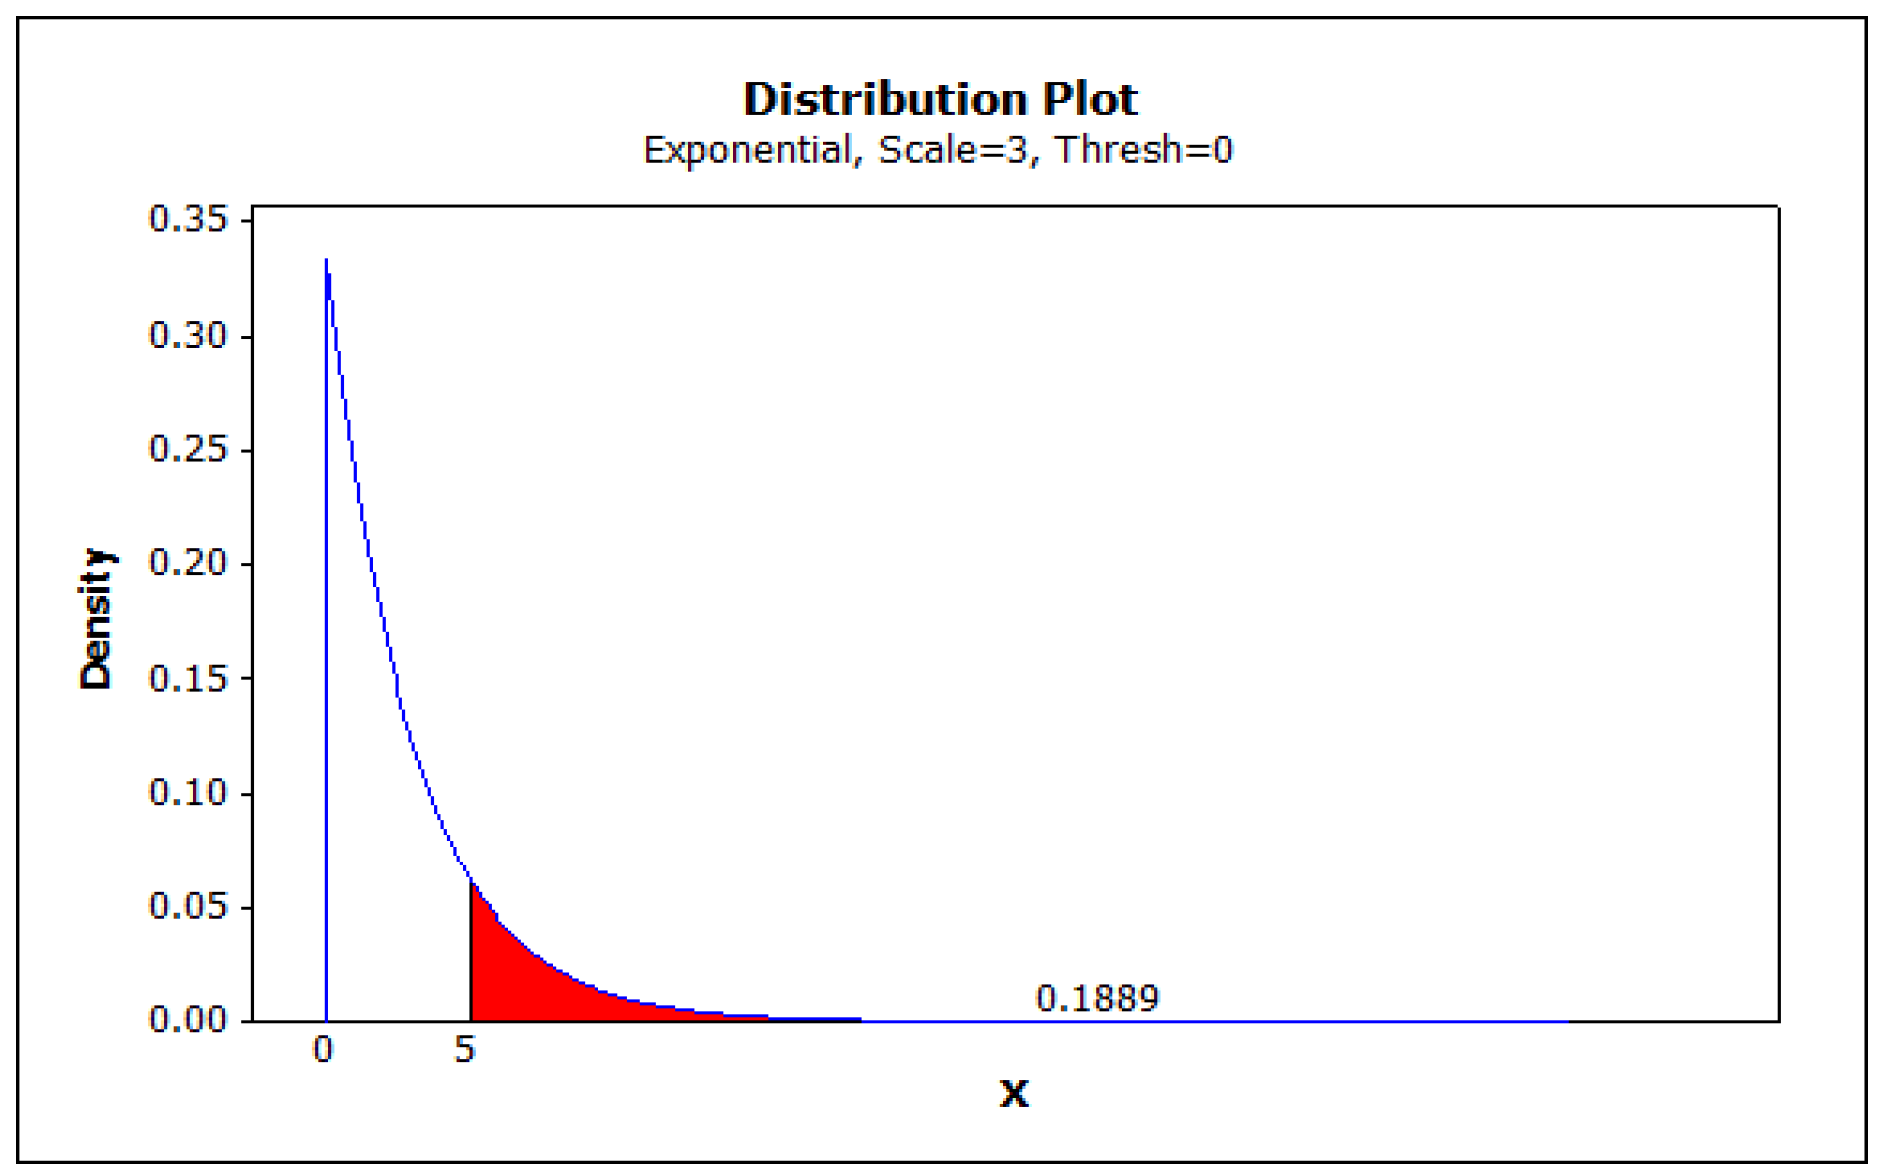
\includegraphics[scale=.15]{figs/pdf_Exponential_density2.png}
% \end{center}
% }
 }
\end{minipage}
}
\end{frame}


\begin{frame}\frametitle{Backward Normal calculations and Percentiles}
\qBrd{teal!40}{We could find the observed value (x) of a given proportion or percentile in Normal$(\mu,\sigma^2)$ by unstandardizing the z-value as follows:
\vspace{-.1in}
\begin{enumerate}
\item Find the z-value corresponding to the lower tail probability using $\Phi^{-1}(\cdot)$
\item Unstandardize $x=\mu+\sigma z$.
\end{enumerate}
}

\vspace{.1in}
\qBrd{applegreen!40}{
\sqBullet{applegreen} In the standard normal distribution, z will denote the z-value for
which of the area under the standard normal curve lies to the right of z,  i.e. $P(Z\geq z_{\alpha})=\alpha$
\vspace{-.3in}
\begin{center}
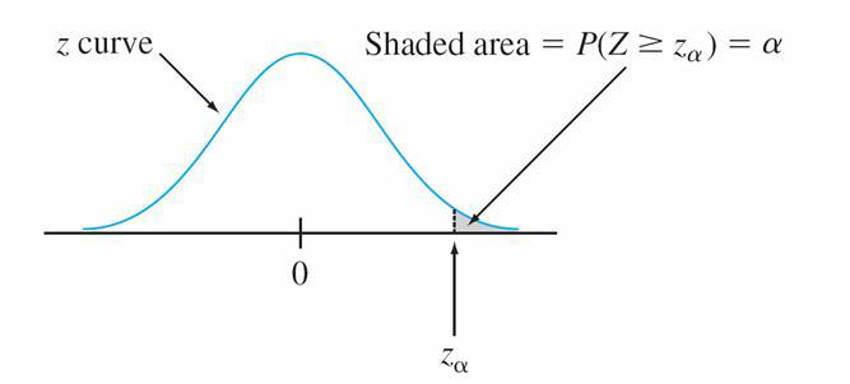
\includegraphics[scale=.4]{figs/Normal_Cutoff.png}
\end{center}
}

\end{frame}






\begin{frame}\frametitle{Example}
%\tiny
\vspace{-.1in}
\qbx[4.6in]{olive!40}{\small
\Exmpl{olive}{} The times of first failure of a unit of a brand of ink jet printers are approximately normally distributed with a mean of 1,500 hours and a standard deviation of 200 hours. Use the statistical calculator.
\begin{enumerate}[a).]
\item what should be the guarantee time for these printers if the manufacturer wants only 5\% to fail within the guarantee period.
\end{enumerate}
}\\
%\pause

{\tiny 
\begin{minipage}{.45\textwidth} %
{\tiny 
$X\sim$ Normal$(\mu = 1500, \sigma^2=200^2).$ Now we want to find $a$ such that $P(X <a) = 0.05$, so\\
 \qBrd[2in]{babyblueeyes!40}{
 \vspace{-.1in}
\begin{eqnarray*}
& & P(X<a)=0.05\\
& \implies&  P(\HLTY{\frac{X-\mu}{\sigma}}<\frac{a-\mu}{\sigma})=0.05\\
&  \implies &   P\left(\HLTY{Z}<\frac{a-\mu}{\sigma}\right)=0.05\\
&  \implies &   \Phi\left( \frac{a-\mu}{\sigma}\right)=0.05\\
&  \implies &   \frac{a-\mu}{\sigma}=\Phi^{-1}\left(0.05\right)\\
&  \implies &  a= \mu +\sigma\Phi^{-1}\left(0.05\right)\\
&  \implies &  a= 1500 +200\times (- 1.64)\\
& =& 1172.
\end{eqnarray*}
\vspace{-.1in}
}
}
\end{minipage} % 
\hspace{.1in}
\begin{minipage}{.45\textwidth} %
{\tiny 
% \qBrd[2.1in]{babyblue!40}{\begin{center}
% %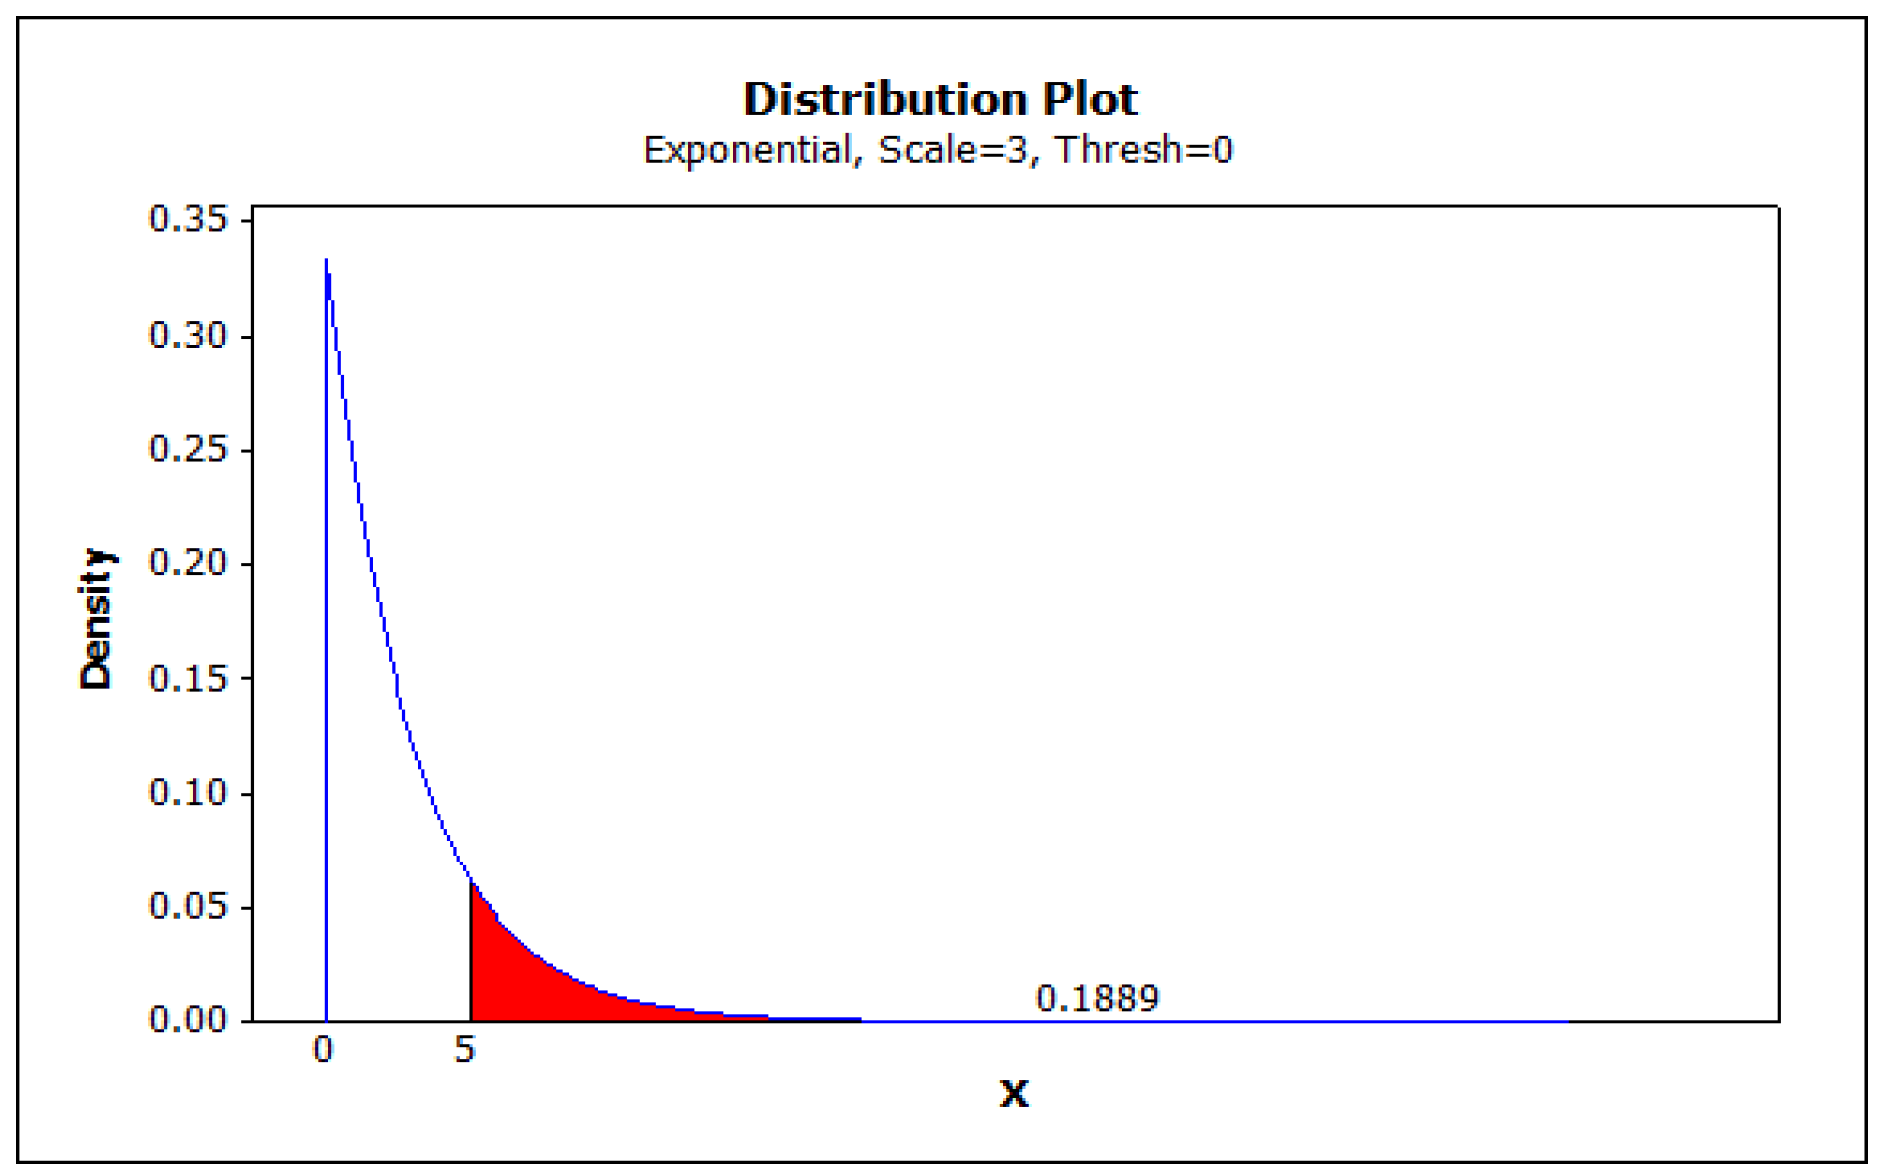
\includegraphics[scale=.15]{figs/pdf_Exponential_density2.png}
% \end{center}
% }
 }
\end{minipage}
}
\end{frame}






\begin{frame}\frametitle{Exercise}
%\tiny
\vspace{-.1in}
\qbx[4.6in]{teal!40}{
\Exmpl{teal}{} An engineer working for a manufacturer of electronic components takes a large number of measurements of a particular dimension of components from the production line.  She finds that the distribution of dimensions is normal, with a mean of 2.340 cm and a standard deviation of 0.06 cm.
\begin{enumerate}[a).]
\item What percentage of measurements will be less than 2.45 cm?
\item What percentage of dimensions will be between 2.25 cm and 2.45 cm?
\item What value of the dimension will be exceeded by 98\% of the components?
\end{enumerate}
}\\
%\pause
\vspace{2in}
\end{frame}






\begin{frame}\frametitle{Exercise}
%\tiny
\vspace{-.1in}
\qbx[4.6in]{applegreen!40}{
\Exmpl{applegreen}{} Wires manufactured for use in a computer system are specified to have resistances between 0.12 and 0.14 ohms. The actual measured resistances of the wires produced by company A have a normal probability distribution with mean 0.13 ohm and standard deviation 0.005 ohm.
\begin{enumerate}[a).]
\item What is the probability that a randomly selected wire from company A's production will meet the specifications?
\item If four of these wires are used in each computer system and all are selected from company A, what is the probability that all four in a
randomly selected system will meet the specifications?
\end{enumerate}
}\\
%\pause
\vspace{2in}
\end{frame}




\begin{frame}\frametitle{Exercise}
%\tiny
\vspace{-.1in}
\qbx[4.6in]{amethyst!40}{
\Exmpl{amethyst}{} The SAT and ACT college entrance exams are taken by thousands of students each year. The mathematics portions of each of these exams produce scores that are approximately normally distributed. In recent years, SAT mathematics exam scores have averaged 480 with standard deviation 100. The average and standard deviation for ACT mathematics scores are 18 and 6, respectively.
\begin{enumerate}[a).]
\item An engineering school sets 550 as the minimum SAT math score for new students. What percentage of students will score below 550 in a typical year?
\item  What score should the engineering school set as a comparable standard on the ACT math test?
\end{enumerate}
}\\
%\pause
\vspace{2in}
\end{frame}





\begin{frame}\frametitle{Exercise}
%\tiny
\vspace{-.1in}
\qbx[4.6in]{babyblue!40}{
\Exmpl{babyblue}{} Of the Type A electrical resistors produced by a factory, 85\% have resistance greater than 41 ohms, and 3.7\% of them have resistance greater than 45 ohms. The resistances follow a normal distribution.
\begin{enumerate}[a).]
\item What percentage of these resistors have resistance greater than 44 ohms?
\end{enumerate}
}\\
%\pause
\vspace{2in}
\end{frame}




%\section{Moment Generating Function}
%\TransitionFrame[airforceblue]{\Large Simulations  }
%
%
%\section{Moment Generating Function}
%\TransitionFrame[airforceblue]{\Large Moment Generating Function  }

%\TransitionFrame[airforceblue]{\Large  A }





\TransitionFrame[antiquefuchsia]{\Large Questions?  }
 
 
\end{document}
